\chapter{Oscilloscope: implementation}
    The following chapter gives a more technical description of the internals of the oscilloscope.
    \begin{itemize} 
        \item We provide a more in-depth look at the $\Delta$QSD concepts introduced in the previous chapter.
        \item We then explain how the $\Delta$Q adapter works, its API and the underlying mechanism that let us export outcome instances to the oscilloscope.
        \item Lastly, we briefly talk about the parser generator used to parse the outcome diagram syntax and the dashboard graphical framework.
    \end{itemize}

    \section{$\Delta$QSD implementation}
    A probe's $\Delta$Q can be represented internally by a PDF and displayed as an CDF. Here is how both can be calculated given $n$ outcome instances.
    
    \subsection{Histogram representation}
        The $\Delta$Q representation is one of a histogram for its PDF and a cumulative histogram for its CDF.
    \subsubsection{PDF}
  We approximate the PDF of the observed $\Delta$Q via a histogram. We partition the values into $N$ bins of equal width, Given $\lbrack x_i, x_{i+1} \rbrack$ the interval of a bin $i$, where $x_i = i\Delta t$, and $\hat{p}(x_i)$ the value of the PDF at bin $i$, for $n$ bins:
        \begin{equation}
            \begin{cases}
                \hat{p}(i) = \dfrac{s_i}{n}, \text{if } i \le n \\
                \hat{p}(i) = 0, \text{if } i > n \\
            \end{cases}
            \label{eq:pdf}
        \end{equation}
    Where $s_i$ the number of successful outcome instances whose elapsed time is contained in the bin $i$, $n$ the total number of instances. \cite{stat}

    \subsubsection{CDF}
        The value $x_i = \hat{f}(i)$ of the CDF at bin $i$ with $n$ bins can be calculated as:
        \begin{equation}
            \begin{cases}
                \hat{f}(i) = \sum_{j=1}^{i} \hat{p}(j), & \text{if } i \le n \\  
                \hat{f}(i) = \hat{f}(n), & \text{if } i > n 
            \end{cases}
            \label{eq:cdf}
        \end{equation}
 
    \begin{figure}[H]
            \begin{center}
                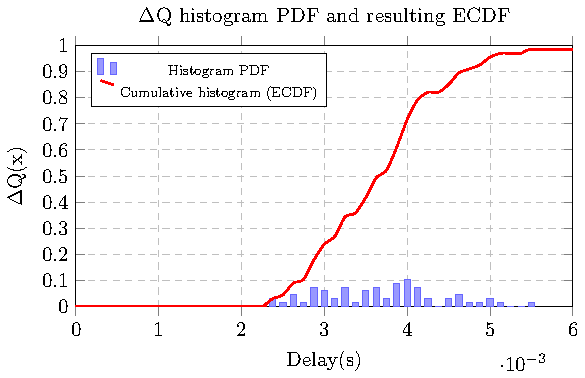
\includegraphics[scale=1]{tikz/pdf_dq.pdf} 
            \end{center}
            \caption{Blue bins: PDF of a sample $\Delta$Q. Red: Resulting CDF of $\Delta$Q PDF, the CDF is what is displayed on the dashboard.}
        \end{figure}

    \subsection{dMax}
        We introduced $dMax$ in the previous chapters, we provide here the full equation that allows $dMax$ to be calculated:
        \begin{equation}
            dMax = \Delta t_{base} * 2^n * N  
            \label{eq:dMaxU}
        \end{equation}
        Where:
        \begin{itemize}
            \item $\Delta t_{base}$ represents the base width of a bin, equal to 1ms.
            \item $n$ the exponent that is set by the user in the dashboard. It is limited to [-10, 10].
            \item $N$ the number of bins.
        \end{itemize}
            We chose 1 ms in combination with $2^n$ as it allows us to go from very fine bin widths ($\approx$ 1 $\mu$) to large bin widths ($\approx$ 1 s) 
    \subsection{Convolution} \label{convol}
    We present the two solution to perform convolutions we explored during the implementation.  
        \subsubsection{Naïve convolution}
        Given two $\Delta$Q binned PDFs $f$ and $g$ with equal bin widths, the result of the convolution $f \circledast g$ is given by \cite{conv}: 
        \begin{equation}
            (f \circledast g)\lbrack n \rbrack = \sum_{m = 0}^{N} = f\lbrack m \rbrack g \lbrack n - m \rbrack  
            \label{eq:discconv}
        \end{equation}

        The naïve way of calculating convolution has a time complexity of $\mathcal{O}(N^2)$, this quickly becomes a problem as soon as the user wants to have a more fine-grained understanding of a component. Moreover, the oscilloscope started presenting noticeable lag and frame skipping. This is why we decided to explore Fast Fourier Transform convolution. 
 
    \subsubsection{Fast Fourier Transform Convolution}
        FFTW (Fastest Fourier Transform in the West) is a C subroutine library \cite{fftw3} for computing the discrete Fourier Transform in one or more dimensions, of arbitrary input size, and of both real and complex data. We use FFTW in our program to compute the convolution of $\Delta$Qs. We adapt our script from an already existing one found on GitHub. \cite{fft}
    
    Whilst the previous algorithm is far too slow to handle a high number of bins, convolution leveraging Fast Fourier Transform (FFT) allows us to reduce the amount of calculations to $\mathcal{O}(N \text{log} N)$. This is why the naïve convolution algorithm is not used. We will analyse the time gains in a later chapter.
    
    FFT and naïve convolution produce the same results in our program, barring $\varepsilon$ differences (around $10^{-18}$) in bins whose result should be 0. This is most likely due to rounding error.
    
    FFTs algorithms are plenty, the choice of the one to use is left up to the subroutine via the parameter \texttt{FFTW\_ESTIMATE} \cite{fft-h}.

    \subsection{Arithmetical operations}
        The FTF, ATF and PC operators on $\Delta$Qs use a simple set of arithmetical operations to calculate a $\Delta$Q.   
    The time complexity of FTF, ATF and PC is trivially $\mathcal{O}(N)$ where N is the number of bins.
 
    \paragraph{Scaling (multiplication)} A $\Delta$Q can be scaled w.r.t. a constant $0 \le j \le 1$. It is equal to binwise multiplication on CDF bins. It is used for the probabilistic choice operator.
    \begin{equation}
        \hat{f_r}(i) = \hat{f}(i) \cdot j
        \label{eq:mul_ecdf}
    \end{equation}

    \paragraph{Operations between $\Delta$Qs} 
        Addition, subtraction and multiplication can be done between two $\Delta$Q of equal bin width (but not forcibly of equal length) by calculating the operation between the two CDFs of the $\Delta$Qs:
        \begin{equation}
            \Delta \text{Q}_{AB}(i) = \hat{f_A}(i) [\cdot, +, -] \hat{f_B}(i)
            \label{eq:op_dq}
        \end{equation}
    They are used for all operators.

    \subsection{Confidence bounds}
        Here is how we calculate the mean and lower/upper confidence for the $\Delta$Qs CDF at bin $i \quad \forall i < N$. \cite{stat}

        For $x_{ij}$ the value of an CDF $j$ at bin $i$, the mean of all CDFs for the bin over a window is:
            \begin{equation}
                \mu_i = \dfrac{1}{n_i} \sum_{j=1}^{n_i} x_{ij}
                \label{eq:mean_ecdf}
            \end{equation}
        Its variance:
            \begin{equation}
                \sigma^2_i = \dfrac{1}{n_i} \sum_{j=1}^{n_i} x^2_{ij} - \mu^2_i
                \label{eq:var_ecdf}
            \end{equation}
        The confidence intervals $CI_i$ for a bin $i$ can then be calculated as:
        \begin{equation}
            CI_i = \mu_i \pm \dfrac{\sigma_i}{\sqrt{n_i}}      
            \label{eq:ci_i}
        \end{equation}

        \subsection{Rebinning}
            Rebinning refers to the aggregation of multiple bins of a bin width $i$ to another bin width $j$. 
            Previous operations between $\Delta$Qs must be done on $\Delta$Qs that have the same bin width. This is why it is fundamental that all probes have a common $\Delta t_{base}$ and why we have a $2^n$ factor to calculate the total bin width.

            Given two $\Delta$Qs $\Delta$Q$_i$, $\Delta$Q$_j$, the common bin width $\Delta t_{ij}$ is:
            \begin{center}
                $\Delta t_{ij}$ = max \{$\Delta_{Ti}, \Delta_{Tj} \}$
            \end{center}
            and the PDF of the rebinned $\Delta$Q at bin $b$, from the original PDF of $n$ bins, where $k$ = $\frac{\Delta{_Ti}}{\Delta_{Tj}}$:
            \begin{equation}
                p'_b = \sum_{n=b \cdot k}^{b+ 1 \cdot k - 1} p_n, \quad b=0,1,\dots \lceil \frac{N}{k} \rceil  
            \end{equation}
            We perform rebinning to a higher bin width for a simple reason. While this leads to loss of information for the $\Delta$Q with the lowest bin width, rebinning to a lower bin width would imply inventing new values for the $\Delta$Q with the highest bin width.
        \begin{figure}[H]
            \centering
            \begin{subfigure}{.5\textwidth}
                \centering
                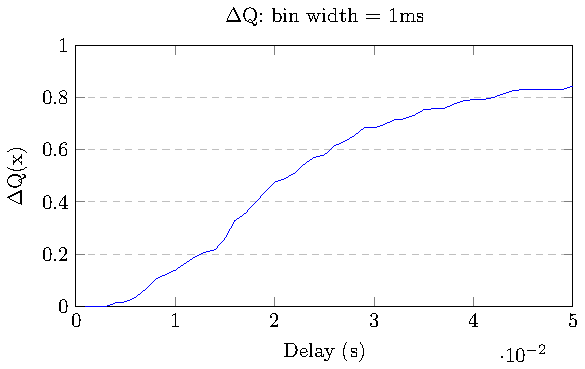
\includegraphics[width =0.98\textwidth]{tikz/cdf.pdf}
                \label{fig:nrb}
                \subcaption{Sample $\Delta$Q with 1ms bins}%
            \end{subfigure}%
            \begin{subfigure}{.5\textwidth}%
                \centering%
                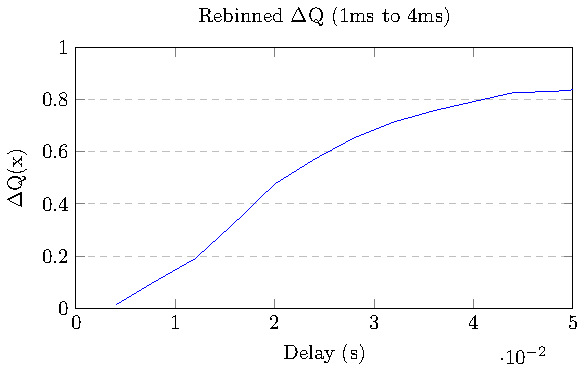
\includegraphics[width =0.98\textwidth]{tikz/rebinned_cdf.pdf}%
                \label{fig:sub2}%
                \subcaption{$\Delta$Q on the left after rebinning to 4ms bins}%
            \end{subfigure}%
            \label{fig:w1w2hb}%
            \end{figure}%



    \section{Adapter}
    The adapter, called \texttt{dqsd\_otel} is a rebar3 \cite{rebar3} application built to replace OpenTelemetry calls and create outcome instances, it is designed to be paired with the oscilloscope to observe an Erlang application.
    
    \subsection{API}
        The adapter functions to be used by the user are made to replace OpenTelemetry calls to macros as for \texttt{?start\_span} and \texttt{?with\_span} and \texttt{?end\_span}. This is to make the adapter less of an encumbrance for the user. 

        Moreover, the adapter will always start OpenTelemetry spans but only start outcome instances if the adapter has been activated. The adapter can be activated by the oscilloscope by pressing the "start adapter" button and can be stopped via the "stop adapter" button.
         
        \subsubsection{start\_span/1, start\_span/2}
        
        \begin{minted}{erlang}        
start_span/1: -spec start_span(binary()) -> {opentelemetry:span_ctx(), pid() | ignore}.
start_span/2: -spec start_span(binary(), map()) -> {opentelemetry:span_ctx(), pid() | ignore}.  
        \end{minted}
        
        \paragraph{Parameters:}
        \begin{itemize}
            \item Name: Binary name of the probe.
            \item Attributes: The OpenTelemetry span attributes (Only for start\_span/2).
        \end{itemize} 
        
        \texttt{start\_span} incorporates OpenTelemetry \texttt{?start\_span(Name)} macro.
        
        \paragraph{Return:} 
        The function returns either:
        \begin{itemize}
            \item  \texttt{\{SpanCtx, span\_process\_PID\}} if the adapter is active and the probe's $dMax$ has been set.
            \item \texttt{\{SpanCtx, ignore\}} if one of the two previous conditions was not respected.
        \end{itemize}
        With SpanCtx being the context of the span created by OpenTelemetry.
        
        \subsubsection{with\_span/1, with\_span/2}
        
        \begin{minted}{erlang}
with_span/1: -spec with_span(binary(), fun(() -> any())) -> any().
with_span/2: -spec with_span(binary(), map(), fun(() -> any())) -> any().
        \end{minted}
         
        \paragraph{Parameters:}
            \begin{itemize}
                \item Name: Binary name of the probe.
                \item Fun: Zero-arity function representing the code of block that should run inside the \texttt{?with\_span} macro.
                \item Attributes: The OpenTelemetry span attributes (Only for with\_span/3).

            \end{itemize}

        \texttt{with\_span} incorporates OpenTelemetry \texttt{with\_span} macro. \\
        \paragraph{Return:}
            \texttt{with\_span} returns what \texttt{Fun} returns (\texttt{any()}).
        
        \subsubsection{end\_span}
            \begin{minted}{erlang}                
-spec end_span(opentelemetry:span_ctx(), pid() | ignore) -> ok | term().
            \end{minted}
            \paragraph{Parameters:}
            \begin{itemize}
                \item SpanCtx: The context of the span returned by \texttt{start\_span}.
                \item Pid: \texttt{span\_process\_PID} || \texttt{ignore}.
            \end{itemize}

    As is the case for \texttt{start\_span}, \texttt{end\_span} incorporates an OpenTelemetry macro, in this case \texttt{?end\_span(Ctx)}. \\

        \subsubsection{fail\_span}
        \begin{minted}{erlang}        
-spec fail_span( pid() | ignore) -> ok | term().
        \end{minted}
        \paragraph{Parameter:}
             \begin{itemize}
                \item Pid: \texttt{ignore} || \texttt{span\_process\_PID}.
            \end{itemize}
            \texttt{fail\_span} does not incorporate any OpenTelemetry macro, it is let up to the user to decide how to handle failures in execution. \\
        

        \subsubsection{span\_process}
            \texttt{span\_process} is the process, spawned by \texttt{start\_span}, responsible for handling the \texttt{end\_span, fail\_span, timeout} messages.

            Upon being spawned, the process starts a timer with time equal to the $dMax$ set by an user for the probe being observed, thanks to \texttt{erlang:send\_after}. When the timer runs out, it sends a \texttt{timeout} message to the process.
        
        The process can receive three kinds of messages:
        \begin{itemize}
            \item \texttt{\{end\_span, end\_time\}}: This will send a custom span to the oscilloscope with the start and end time of the execution of the probe.
            \item \texttt{\{fail\_span, end\_time\}}: This will send a custom span to the oscilloscope indicating that an execution of a probe has failed.
            \item \texttt{\{timeout, end\_time(StartTime + $dMax$)\}}: If the program hasn't ended the span before $dMax$, the timer will send a \texttt{timeout} message and it will send an outcome instance to the oscilloscope indicating that an execution of a probe has timed out.
        \end{itemize}
        The process is able to receive one and only message, if the execution times out and subsequently the span is ended, the oscilloscope will not be notified as the process is defunct. This is assured by Erlang documentation:
        \begin{center}
            \textit{If the message signal was sent using a process alias that is no longer active, the message signal will be dropped.} \cite{erl-s}
        \end{center}

    \subsection{Handling outcome instances}
        To create outcome instances of a probe we must obtain three important informations:
        \begin{itemize}
            \item Its name.
            \item The time when the span was started.
            \item Its $dMax$.
        \end{itemize}
        
        They start time and end time are supplied by calling this function:
        \begin{minted}{erlang}
        StartTime/EndTime = erlang:system_time(nanosecond).
        \end{minted}
        The name is given when starting a span and the $dMax$ is stored in a dictionary in the adapter. 

            The outcome instance is created only if two conditions are met: the adapter has been set as active and the user set a timeout for the probe, the functions will spawn a \texttt{span\_process} process, passing along all the necessary informations. \\
        Once the span is subsequently ended/timed out/failed, the function \texttt{send\_span} creates a message carrying all the informations and sends it to the C++ server. The formatting of the messages is the following:
        \begin{minted}{text}
            n:Observed name, b: Start time (beginning), e: End time (end or deadline), s: The status
        \end{minted}

    \subsection{TCP connection}
        The adapter is composed of two \texttt{gen\_server} which handle communication to and from the oscilloscope. This gen\_server behaviour allows the adapter to send spans asynchronously to the oscilloscope.

        \subsubsection{TCP server}
            The TCP server is responsible for receiving commands from the oscilloscope. It can be run by setting its IP and port via:
            \begin{minted}{erlang}
                -spec start_server(string() | binary() | tuple(), integer()) -> ok | {error, Reason}
            \end{minted}
            The oscilloscope can send commands to the adapter, these commands are:
            \begin{itemize}
                \item \texttt{start\_stub}: This command sets the adapter as active, it can now send outcome instances to the oscilloscope if the probe's $dMax$s are defined.
                \item \texttt{stop\_stub}: This commands sets the adapter as inactive, it will no longer send outcome instances to the oscilloscope.
                \item \texttt{set\_timeout;probeName;timeout}: This command indicates to the adapter to set the $dMax = \text{timeout}$ for a probe, a limit of the adapter is that erlang:send\_after does not accept floats as timeouts, so the timeout will be rounded to the nearest integer.
            \end{itemize}

        \subsubsection{TCP client}
            The TCP client allows the adapter to send the spans to the oscilloscope.
            The client connects over TCP to the oscilloscope by connecting to the oscilloscope server's address and opens a socket where it can send the outcome instances.
            \begin{minted}{erlang}
                -spec try_connect(string() | binary(), integer()) -> ok.
            \end{minted}

    \section{Parser}
        To parse the system, we use the C++ ANTLR4 (ANother Tool for Language Recognition) library \cite{antlr4}. 
        \subsection{ANTLR}
    According to ANTLR website \cite{antlr4}: 
    \begin{quote}
        ANTLR is a parser generator for reading, processing, executing or translating structured text files. ANTLR generates a parser that can build and walk parse trees.
    \end{quote}

 ANTLR is just one of the many parsers generators available in C++ (flex/bison \cite{flexb}, lex/yacc \cite{lexy}). Although it presents certain limitations, its generated code is simpler to handle and less convoluted with respect to the other possibilities.

        ANTLR uses Adaptive LL(*) \textit{(ALL(*))} parser, namely, it will ``move grammar analysis to parse-time, without the use of static grammar analysis''. \cite{antlr}

        \subsection{Grammar}
            ANTLR provides a yacc-like metalanguage \cite{antlr} to write grammars. The grammar we have written can be found in the appendix \ref{code:grammar}.
              
    \subsubsection{Limitations}
        A previous version was implemented in Lark \cite{lark}, a python parsing toolkit. The python version was quickly discarded due to a more complicated integration between Python and C++. Lark provided Earley(SPPF) strategy which allowed for ambiguities to be resolved, which is not possible in ANTLR. \\
        For example the following system definition presents a few errors:
        \begin{minted}{text}
        probe = s -> a -> f -> p;
        \end{minted}
    While Lark could correctly guess that everything inside was an outcome, ANTLR expects \texttt{``:''} after ``s, a, f'' and ``p'', thus, one can not name an outcome by these characters, as the parser generator thinks that an operator or a probe will be next. 

    \section{Oscilloscope GUI}
    Our oscilloscope graphical interface has been built using the QT framework for C++. Qt is ``a cross-platform application development framework for creating graphical user interfaces'' \cite{qt-w}. We chose Qt as we believe that it is the most documented and practical library for GUI development in C++. Using Qt allows us to create usable interfaces quickly, while being able to easily pair the backend code of C++ to the frontend.

    The interface is composed of a main window, where widgets can be attached to it easily. Everything that can be seen is customisable widgets. This allows for easy reusability, modification and removal without great refactoring due in other parts of the system. We provide a screenshot of the ``widget view'' in \cref{app:dash_wid}.


